\documentclass[a4paper]{article}

\usepackage[spanish]{babel}
\usepackage[utf8]{inputenc}
\usepackage{graphicx}
\usepackage{amsmath}
\usepackage[T1]{fontenc}
\usepackage{hyperref}
\usepackage{float}


\title{Proyecto de investigación sobre detección de caras mediante OpenCV} 
\author{Alejandro Rodríguez Rodríguez \and Pablo Cano Navajas \and Salvador Caballero Macías}

\begin{document}

\maketitle

\newpage
\tableofcontents

\newpage
\section*{Resumen}

Este documento detalla las diferentes implementaciones que se han llevado a cabo durante la implementación de las mismas, asi como los resultados obtenidos y las conclusiones a las que se ha llegado. El proyecto se ha realizado empleando el repositorio\cite{1} que se detalla en el libro escogido\cite{2}.
De la documentacion escogida, se ha seleccionado el capítulo número 5, que trata sobre la detección de caras, tanto en imágenes como en captura en tiempo real, así como las implementaciones de mejoras de los algoritmos que se tratan en el libro para detectar un mayor número de caras o distintos objetos que cumplan unas restricciones que se impongan.

\section{Introducción}

El capítulo 5 del libro \textit{Learning OpenCV 4 Computer Vision with Python 3 Third Edition} \cite{2} se centra en la \textbf{detección y reconocimiento de caras}. Este capítulo introduce la funcionalidad de OpenCV para estas tareas, junto con los archivos de datos que definen tipos particulares de objetos rastreables. Se exploran los \textbf{clasificadores de cascada Haar}, que analizan el contraste entre regiones de imagen adyacentes para determinar si una imagen o subimagen coincide con un tipo conocido.

Un método clásico y ampliamente utilizado
para la detección de rostros es el uso de clasificadores en cascada de Haar,
implementados eficientemente en bibliotecas como OpenCV. Estos clasificadores
analizan el contraste entre regiones adyacentes de una imagen mediante un
conjunto de características similares a Haar organizadas en una estructura en
cascada para una rápida evaluación de posibles regiones de rostro. 
\begin{figure}[h!]
    \centering
    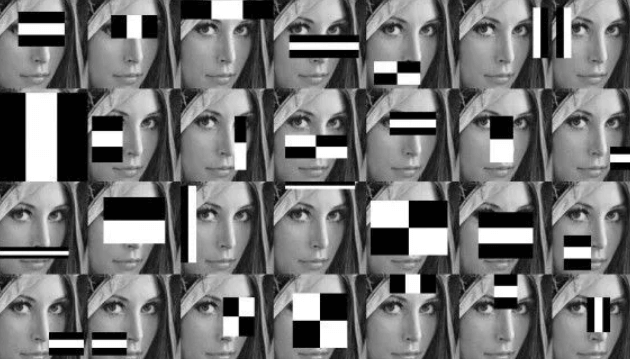
\includegraphics[width=0.6\textwidth]{../img/haar_cascade.png}
    \caption{Ejemplo de características Haar en una imagen.}
\end{figure}

Si bien esta
técnica ha demostrado ser efectiva en muchas situaciones, su rendimiento puede
verse afectado por diversos factores, como la escala, la orientación y las condiciones
de detección. En este trabajo, exploramos una mejora en la detección
de rostros utilizando los clasificadores en cascada de Haar mediante la optimizaci
ón de los parámetros del proceso de detección, buscando un equilibrio entre
la sensibilidad del detector y la reducción de falsos positivos.

\section{Planteamiento teórico}

En esta sección se detalla el planteamiento teórico del capítulo 5 del libro\cite{1}, que se centrará en los fundamentos de las cascadas de Haar mediante el uso de OpenCV para la detección de caras. Se dividirá en 3 subapartados, correspondientes a los subapartados del propio capítulo:

Los clasificadores en cascada de Haar funcionan mediante la aplicación de
una serie de clasificadores, cada uno entrenado para descartar la mayoría de
las regiones negativas mientras retiene las regiones que contienen el objeto de
intés (en este caso, rostros). Estos clasificadores se basan en la evaluación
de características simples, computacionalmente eficientes, que codifican diferencias
en la intensidad de píxeles entre regiones rectangulares adyacentes. Para
detectar rostros en imágenes de diferentes tamaños, se emplea una ventana de
detección que se desliza sobre la imagen a diferentes escalas, generando múltiples
subventanas para su análisis.
\begin{figure}[!h]
    \centering
    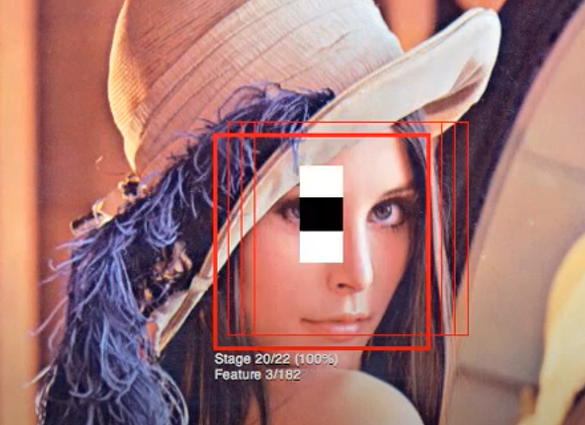
\includegraphics[width=0.6\textwidth]{../img/haar_iter.png}
    \caption{Ejemplo de iteración sobre características de una cara.} (\textit{Ver anexo 1}).
\end{figure}

En OpenCV, la detección de múltiples escalas de rostros se implementa
mediante la función detectMultiScale del objeto cv2.CascadeClassifier.
Esta función toma como entrada una imagen y varios parámetros que controlan
el proceso de búsqueda de objetos. Dos de los parámetros más influyentes en el
rendimiento del detector son scaleFactor y minNeighbors.

\subsection{Conceptualizando las Cascadas de Haar}

El concepto de clasificación de objetos y el seguimiento de su ubicación buscan identificar qué constituye una parte reconocible de un objeto. Las imágenes fotográficas pueden contener muchos detalles, pero estos detalles pueden ser inestables debido a variaciones en la iluminación, el ángulo de visión, la distancia de visión, el movimiento de la cámara y el ruido digital. Afortunadamente, para la clasificación, no todas las diferencias en los detalles físicos son relevantes.

Las \textbf{características tipo Haar} son un tipo de característica que se aplica a menudo a la detección de rostros en tiempo real. 
\begin{figure}[h!]
    \centering
    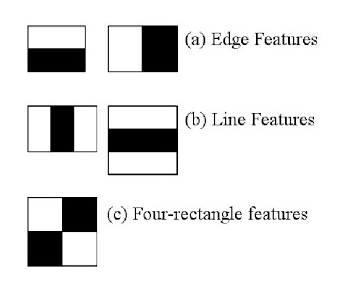
\includegraphics[width=0.6\textwidth]{../img/haar_feat.png}
    \caption{Tipos de características de Haar.}
\end{figure}

Estas características describen el patrón de contraste entre regiones de imagen adyacentes. Por ejemplo, los bordes, los vértices y las líneas delgadas generan un tipo de característica. Algunas características son distintivas en el sentido de que típicamente ocurren en una cierta clase de objeto (como una cara) pero no en otros objetos. Estas características distintivas se pueden organizar en una jerarquía, llamada \textbf{cascada}, en la que las capas superiores contienen características de mayor distinción, lo que permite que un clasificador rechace rápidamente los sujetos que carecen de estas características.

Las características pueden variar según la escala de la imagen y el tamaño del vecindario dentro del cual se evalúa el contraste, llamado \textbf{tamaño de ventana}. 

\begin{figure}[H]
    \centering
    \begin{minipage}[b]{0.32\textwidth}
        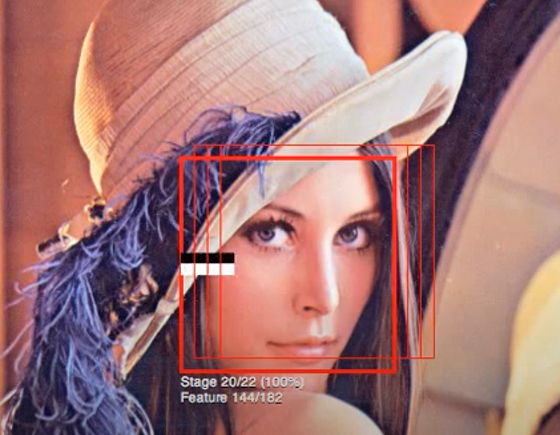
\includegraphics[width=\textwidth]{../img/hf1.png}
    \end{minipage}
    \hfill
    \begin{minipage}[b]{0.32\textwidth}
        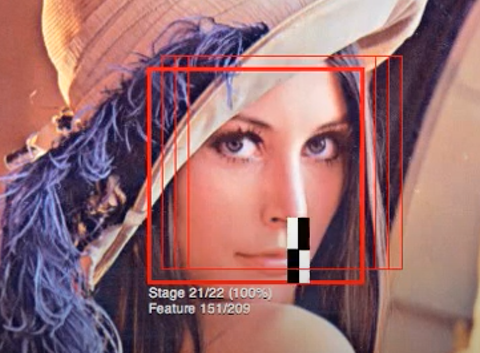
\includegraphics[width=\textwidth]{../img/hf2.png}
    \end{minipage}
    \hfill
    \begin{minipage}[b]{0.32\textwidth}
        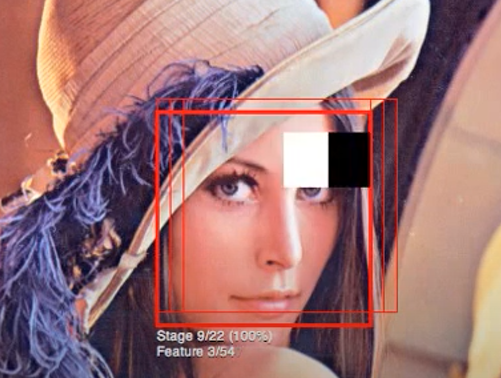
\includegraphics[width=\textwidth]{../img/hf3.png}
    \end{minipage}
    \caption{Ejemplo de características Haar en una imagen.}
\end{figure}

Para hacer que un clasificador de cascada Haar sea \textbf{invariante a la escala}, el tamaño de la ventana se mantiene constante pero las imágenes se reescalan varias veces; de esta manera, a algún nivel de reescalado, el tamaño de un objeto (como una cara) puede coincidir con el tamaño de la ventana. La imagen original y las imágenes reescaladas juntas se denominan \textbf{pirámide de imágenes}, y cada nivel sucesivo en esta pirámide es una imagen reescalada más pequeña. OpenCV proporciona un clasificador invariante a la escala que puede cargar una cascada Haar desde un archivo XML en un formato particular. Internamente, este clasificador convierte cualquier imagen dada en una pirámide de imágenes.

\subsection{Usando OpenCV para la Detección de Caras}

El código fuente de OpenCV 4, o una instalación preempaquetada, debería contener una subcarpeta llamada \texttt{data/haarcascades} . Esta carpeta contiene archivos XML que pueden ser cargados por una clase de OpenCV llamada \texttt{cv2.CascadeClassifier} . Una instancia de esta clase interpreta un archivo XML dado como una cascada Haar, que proporciona un modelo de detección para un tipo de objeto como una cara . \texttt{cv2.CascadeClassifier} puede detectar este tipo de objeto en cualquier imagen, ya sea una imagen fija de un archivo o una serie de fotogramas de un archivo de video o una cámara de video.

Para realizar la detección de caras, se puede crear un script básico que cargue un clasificador de cascada Haar para la detección de rostros y luego aplique este clasificador a una imagen. 

\begin{figure}[h!]
    \centering
    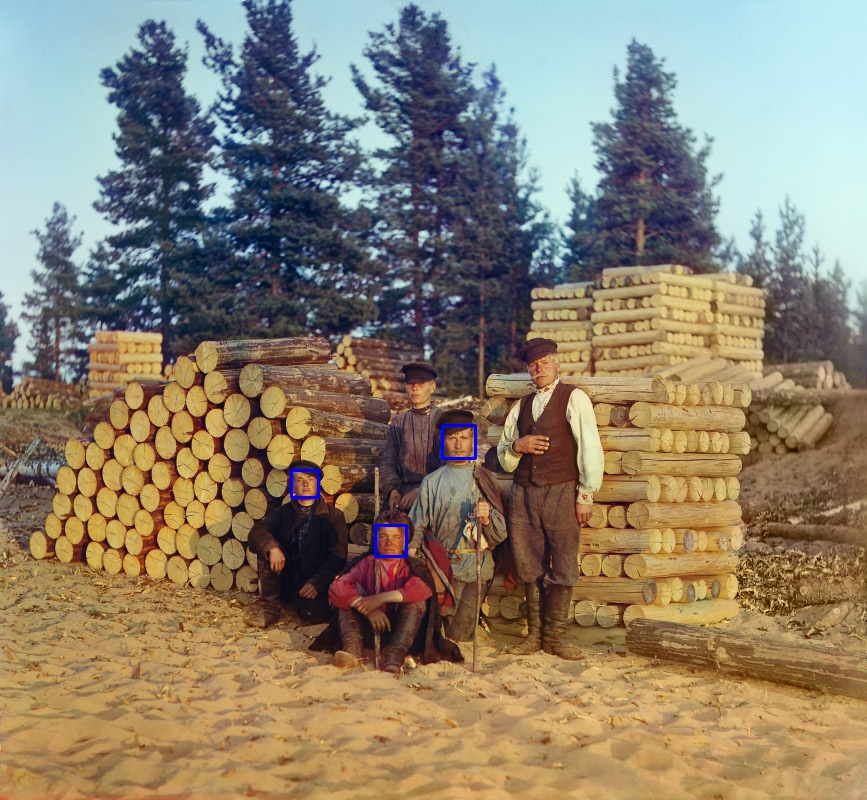
\includegraphics[width=0.6\textwidth]{../img/woodcutters_face_detection.jpg}
    \caption{Ejemplo de detección de caras.}
\end{figure}

\subsection{Mejorando el Clasificador de Cascadas de Haar}

La efectividad de un clasificador de cascada Haar puede verse afectada por los parámetros utilizados en la función \texttt{detectMultiScale}, como los atributos \texttt{scaleFactor} y \texttt{minNeighbors}.
En esta sección se explica cómo detectar caras tanto en imagenes como en una entrada de vídeo en tiempo real (e.g. una cámara de vídeo).
OpenCV proporciona herramientas avanzadas para el procesamiento de imágenes y la detección de objetos mediante el uso de clasificadores en cascada de Haar.\newline

\section{Implementación/Experimentación}

\subsection{Implementación de Cascadas de Haar}

\subsection{Implementación de Detección de Caras}

En el repositorio, dentro de la carpeta faceDetection, podemos encontrar una serie de archivos. El archivo \texttt{0_stillImageFaceDetection} contiene el código para detectar imágenes estáticas con las explicaciones paso a paso del funcionamiento del algoritmo en inglés. Al final de dicho archivo se puede encontrar un apéndice con una explicación más extendida sobre ciertos parámetros o subrutinas de las funciones.

El método clave para realizar la detección de caras es \texttt{detectMultiScale}, que se aplica a una imagen en escala de grises. Los parámetros de \texttt{detectMultiScale} incluyen \texttt{scaleFactor} y \texttt{minNeighbors} (\textit{Ver anexo 2}). El argumento \texttt{scaleFactor}, que debe ser mayor que 1.0, determina la relación de reducción de escala de la imagen en cada iteración del proceso de detección de rostros. El argumento \texttt{minNeighbors} es el número mínimo de detecciones superpuestas que se requieren para conservar un resultado de detección.

También es posible realizar la detección de caras en un video utilizando una cascada Haar para rostros y otra para ojos. El proceso implica capturar fotogramas de una cámara, convertirlos a escala de grises y luego aplicar el detector de rostros. Para cada rostro detectado, se puede definir una región de interés (ROI) y aplicar un detector de ojos dentro de esa ROI.

El \texttt{scaleFactor} influye en la robustez a diferentes tamaños de rostro, mientras que \texttt{minNeighbors} ayuda a reducir los falsos positivos al requerir múltiples detecciones superpuestas. Ajustar estos parámetros mediante experimentación puede mejorar el rendimiento del detector en diferentes condiciones de iluminación y para diferentes sujetos. Además, el uso de múltiples clasificadores en cascada, como uno para la detección frontal de rostros y otro para la detección de ojos dentro de la región facial detectada, puede aumentar la precisión de la detección de características específicas.

\begin{figure}[h!]
    \centering
    \begin{minipage}[b]{0.48\textwidth}
        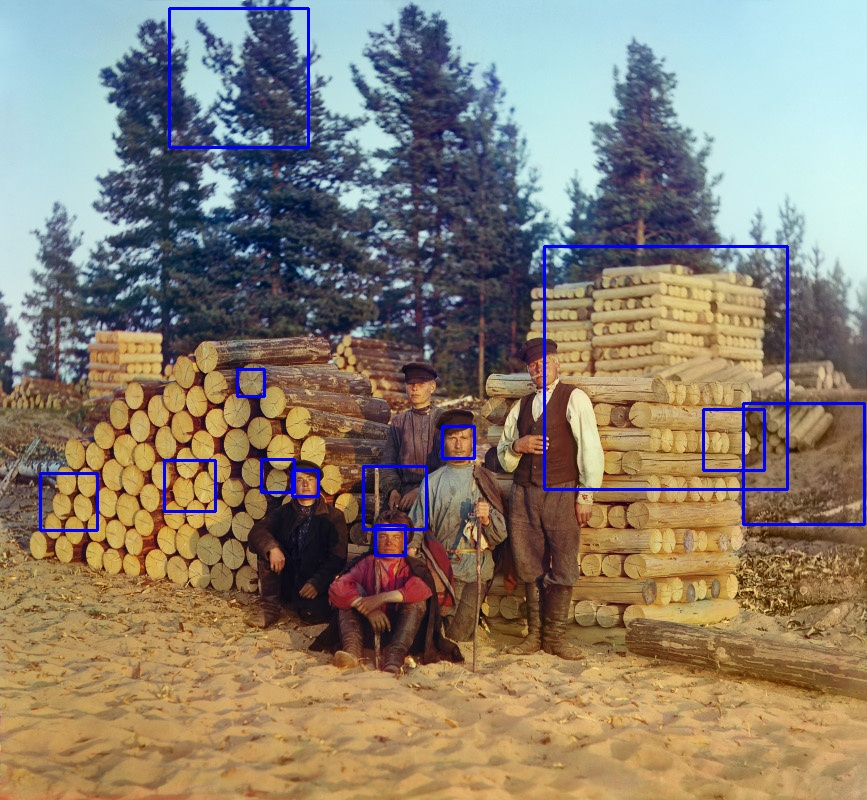
\includegraphics[width=\textwidth]{../img/woodcutters_face_detection103.jpg}
        \caption{Ejemplo de detección con un índice de 1.03}
    \end{minipage}
    \hfill
    \begin{minipage}[b]{0.48\textwidth}
        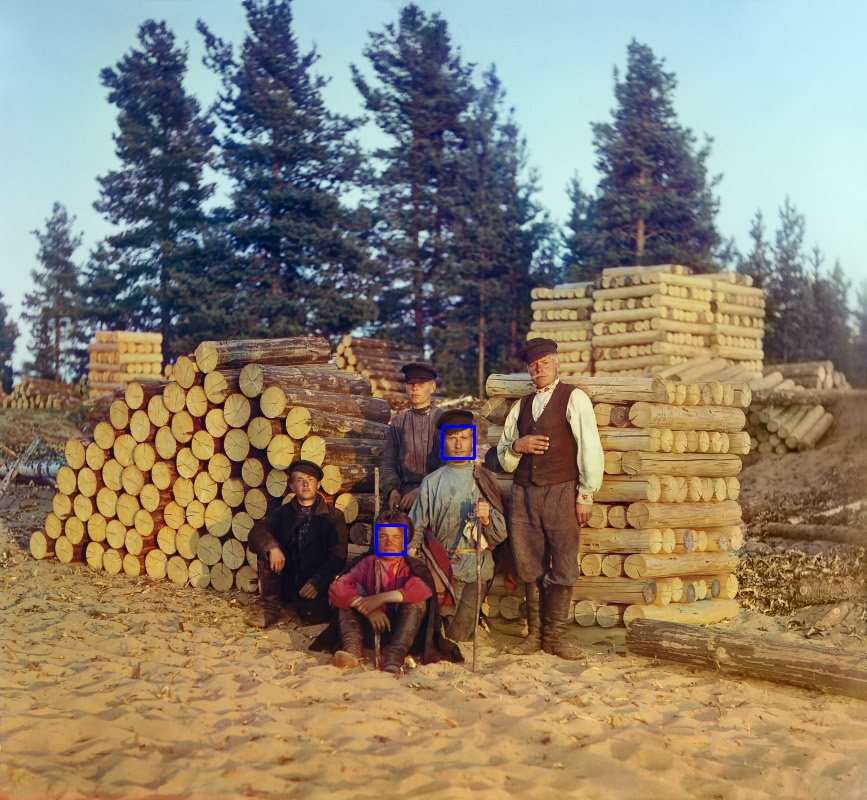
\includegraphics[width=\textwidth]{../img/woodcutters_face_detection11.jpg}
        \caption{Ejemplo de detección con un índice de 1.1}
    \end{minipage}
\end{figure}

Como se puede apreciar en la primera figura, al tener un valor bajo detectará muchos recuadros, dando así falsos positivos. Si aumentamos excesivamente el valor, como se muestra en la figura 7, el algoritmo no detectará correctamente las caras.

Para utilizar un clasificador de cascada Haar en OpenCV para la detección de caras, el primer paso es cargar el archivo XML de la cascada utilizando la función \texttt{cv2.CascadeClassifier()} :

La detección de caras se realiza utilizando archivos XML que contienen los datos preentrenados para identificar características faciales específicas. Estos clasificadores se cargan mediante la función \texttt{cv2.CascadeClassifier}, que permite aplicar los modelos a imágenes o fotogramas de vídeo.
El proceso incluye los siguientes pasos:

\begin{itemize}
    \item Carga de la imagen mediante \texttt{cv2.imread}.
    \item Conversión de la imagen a escala de grises para optimizar el rendimiento del clasificador.
    \item Uso del clasificador \texttt{haarcascade\_frontalface\_default.xml} para detectar caras.
\end{itemize}

// TERMINAR EXPLICACION 1_cameraFaceDetection.ipynb //

El script \texttt{1\_cameraFaceDetection.ipynb} implementa la detección de caras en tiempo real utilizando la cámara del dispositivo. Este proceso incluye:
\begin{itemize}
    \item Captura de vídeo en tiempo real mediante \texttt{cv2.VideoCapture}.
    \item Aplicación del clasificador en cascada a cada fotograma del vídeo.
    \item Detección de características adicionales, como ojos, utilizando el archivo \texttt{haarcascade\_eye.xml}.
\end{itemize}

\subsection{Impementación de Clasificador de Cascada de Haar}

\section{Manual de usuario}

Para el correcto funcionamiento de los scripts, es necessario la instalación de los siguientes paquetes:

\begin{itemize}
    \item \textbf{Windows 7, MacOS 10.7 o superior}.
    \item \textbf{Python 3.8 o superior}. Para instalar Python, se recomienda instalar la versión más reciente accediendo a la página web \href{https://www.python.org/downloads/}{Python.org}. Haremos click en el botón de descarga y se descargará automáticamente el ejecutable. Si fuese necesario otra versión de python, en la misma págna se puede descargar la versión que se necesite.\\
    Si se tiene instalado un sistema operativo distinto a windows, se puede acceder al enlace de \href{https://www.python.org/downloads/macos/}{versiones macOS} y descargar la que sea necesaria siempre que cumppla con los requisitos de instalación.
    \item \textbf{OpenCV 4.0 o superior}. Para instalar la version 4.0 o superior de OpenCV, se recomienda usar el gestor de paquetes \texttt{pip}. Para ello, se abre una terminal y se ejecuta el comando \texttt{pip install opencv-python}. Si la máquina opera con macOS, se recomienda usar \texttt{brew}, escribiendo el comando \texttt{brew install opencv}.
    \item \textbf{NumPy 1.16 o superior}. Para instalarlo, en una ventana de comandos escribiremos \texttt{pip install numpy} (para un entorno Windows) o \texttt{brew install numpy} (para un entorno macOS).
    \item \textbf{Scipy 1.1 o superior}. Para instalarlo, en una ventana de comandos escribiremos \texttt{pip install scipy} (para un entorno Windows) o \texttt{brew install scipy} (para un entorno macOS).

\end{itemize}

\subsection{Instalación de Latex en Visual Studio Code}

Para poder instalar Latex en visual studio code, es necesario instalar los siquientes paquetes:

\begin{itemize}
    \item \textbf{Visual Studio Code}. Para instalarlo, se puede acceder a la página web \href{https://code.visualstudio.com/}{Visual Studio Code} y descargar el instalador correspondiente al sistema operativo que se esté utilizando.
\end{itemize}

\begin{figure}[h!]
    \centering
    
\includegraphics[width=0.6\textwidth]{../img/vsc.png}
    \caption{Página de descarga de Visual Studio Code.}
\end{figure}

\begin{itemize}
    \item \textbf{Latex Workshop}. Para instalarlo, abrimos Visual Studio Code y se accederemos a la pestaña de extensiones (icono de cuatro cuadrados en la barra lateral izquierda). En el campo de búsqueda, escribimos \texttt{latex workshop} y seleccionaremos la opción correspondiente (figura 9). Hacemos click en el botón de instalar.
\end{itemize}

\begin{figure}[h!]
    \centering
    
\includegraphics[width=0.6\textwidth]{../img/extensions.png}
    \caption{Instalación de Latex Workshop.}
\end{figure}

\begin{itemize}
    \item \textbf{MikTeX}. Para instalarlo, se puede acceder a la página web \href{https://miktex.org/download}{MikTeX} y descargar el instalador correspondiente al sistema operativo que se esté utilizando. Una vez descargado, ejecutamos el instalador y seguimos las instrucciones para completar la instalación.
\end{itemize}
    
\begin{figure}[h!]
    \centering
    
\includegraphics[width=0.6\textwidth]{../img/miktex.png}
    \caption{Página de descarga de MikTeX.}
\end{figure}
    

Al final de la instalación se nos preguntará si queremos chequear si hay actualizaciones. Se recomienda chequear la opción para mantenerlo actualizado y evitar errores futuros.
Para crear un nuevo fichero latex, crearemos el fichero con la extensión \texttt{.tex} y lo guardaremos en la carpeta donde se encuentre el proyecto. Para compilar el fichero, haremos click en el icono de \texttt{>} que aparece en el menú de arriba a la derecha en color verde y seleccionaremos la opción de compilar el documento. Esto generará un archivo PDF con el mismo nombre que el archivo \texttt{.tex}.

Es posible que en el proceso de compilación del archivo aparezcan ventanas emergentes pidiendo instalar una serie de paquetes necesarios, instalaremos todos y cuando termine la instalación de todos estos paquetes, se abrirá el archivo compilado en formato PDF. Si no se abre automáticamente, podemos abrirlo manualmente haciendo click en el icono de \texttt{View Latex PDF File} que aparece 2 iconos a la derecha (icono con la lupa) de la opción de compilación (>) como se muestra en la figura 11. Si no aparece, podemos abrirlo manualmente desde la carpeta donde se guardó el archivo \textit{.tex} haciendo click derecho y selecionando la opción \textit{Open to the Side}.

\begin{figure}[h!]
    \centering
    
\includegraphics[width=0.6\textwidth]{../img/menu.png}
    \caption{Opciones del menú de la barra superior.}
\end{figure}

\section{Conclusiones}

\section{Autoevaluación de cada miembro}

\subsection{Autoevaluación de Alejandro}

\subsection{Autoevaluación de Pablo}

\subsection{Autoevaluación de Salvador}

\section{Tabla de tiempos}

\subsection{Tabla de tiempos del grupo}

// RELLENAR //

\subsection{Tabla de tiempos de Alejandro}

// RELLENAR //

\subsection{Tabla de tiempos de Pablo}

\subsection{Tabla de tiempos de Salvador}

\newpage
\begin{thebibliography}{99}
\bibitem{1} \textit{Repositorio del proyecto}, disponible en \href{https://github.com/PacktPublishing/Learning-OpenCV-4-Computer-Vision-with-Python-Third-Edition}{GitHub}
\bibitem{2} Joseph Howse, Joe Minichino, \textit{Learning OpenCV 4 Computer Vision with Python 3}", Third edition, Packt Publishing, pp. 1-372, 2020
\end{thebibliography}

\newpage
\section*{Anexos}
\textbf{|1|} Como se aprecia en la imagen, el cuadrado en rojo indica la posicion de la cara detectada, dentro de este cuadrado se encuentran los elementos de caracteristicas haar, que van iterando sobre la imagen y detectando las facciones de la imagen (tanto ojos, nariz, boca, etc.). En \href{https://youtu.be/hPCTwxF0qf4}{este vídeo} se puede observar como el algoritmo va detectando las facciones.\\

El parámetro \texttt{minNeighbors} es un atributo de detección que establece el número mínimo de detecciones superpuestas requeridas para conservar un resultado de detección. Por ejemplo, un valor bajo (1) puede resultar en más falsos positivos, mientras que un valor más alto (2) reducirá el número de falsos positivos pero puede hacer que se pierdan algunas detecciones.

\end{document}